The equation of a circle can be expressed as,
\begin{align}
    \vec{x}^{T}\vec{x} - 2\vec{c}^{T}\vec{x} +f=0 \label{eq:solutions/7/eq:eq1}
\end{align}
where $\vec{c}$ is the center.\\
Comparing equation \eqref{eq:solutions/7/eq:eq1} with the circle equation given,
\begin{align}
    \vec{x}^{T}\vec{x} =4 \label{eq:solutions/7/eq:eq2}\\
    \implies \vec{c} = \myvec{0\\0} \quad f=-4\\
    r=\sqrt{\vec{c}^{T}\vec{c}-f} = \sqrt{4}\\
    \implies \boxed{r=2} \label{eq:solutions/7/eq:eq3}
\end{align}
From equation \eqref{eq:solutions/7/eq:eq3}, the point at which circle touches $x$-axis is \myvec{2\\0}.\\
The direction vector of $x$-axis is $\myvec{1\\0}$.\\
The direction vector of the given line $\myvec{1&-\sqrt{3}}\vec{x}=0$ is $\myvec{\sqrt{3}\\1}$.\\
The angle that the line makes with the $x$-axis is given by,
\begin{align}
    \cos\theta = \frac{\myvec{\sqrt{3}&1}\myvec{1\\0}}{\norm{\myvec{\sqrt{3}&1}}\norm{\myvec{1&0}}}=\frac{\sqrt{3}}{2} \label{eq:solutions/7/eq:eq4}\\
    \implies \boxed{\theta = 30^{\circ}}\label{eq:solutions/7/eq:eq5}
\end{align}
Using equation \eqref{eq:solutions/7/eq:eq3} and \eqref{eq:solutions/7/eq:eq5},the area of the sector is obtained as,
\begin{align}
    \implies \boxed{\frac{\theta}{360^{\circ}}\pi r^2 = \frac{30^{\circ}}{360^{\circ}}\pi (2)^2=\frac{\pi}{3}} \label{eq:solutions/7/eq:eq6}
\end{align}
\begin{figure}[h!]
	\centering
	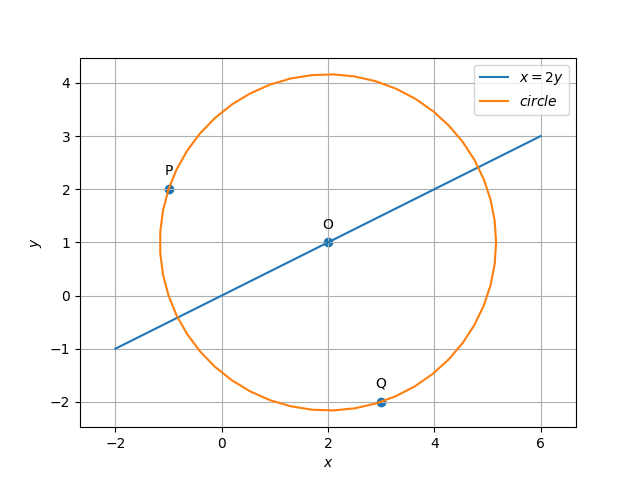
\includegraphics[width=\columnwidth]{./solutions/1/7/circle.png}
	\caption{Region enclosed by $x$-axis, line and circle}
	\label{eq:solutions/7/myfig}
\end{figure}\\
To find points $\vec{A}$ and $\vec{B}$,\\
The parametric form of $x$-axis is,
\begin{align}
    \vec{B} = \vec{q}+\lambda\vec{m}\\
=\myvec{0\\0}+\lambda\myvec{1\\0} \label{eq:solutions/7/eq:eq7}
\end{align}
From the intersection of circle and line, the value of $\lambda$ can be found by,
\begin{align}
    \lambda^2 = \frac{-f_1-\norm{\vec{q}}^2}{\norm{\vec{m}}^2}\\
                = \frac{4-0}{1} = 4\\
    \implies \lambda = \pm{2} \label{eq:solutions/7/eq:eq8}
\end{align}
Sub equation \eqref{eq:solutions/7/eq:eq8} in \eqref{eq:solutions/7/eq:eq7},
\begin{align}
    \vec{B} = \myvec{2\\0}\quad \vec{B} = \myvec{-2\\0} \label{eq:solutions/7/eq:eq9}
\end{align}
As given in question as first quadrant,
\begin{align}
    \implies \boxed{\vec{B} = \myvec{2\\0}} \label{eq:solutions/7/eq:eq10}
\end{align}
Similarly, to find point $\vec{A}$,
The parametric form of line is,
\begin{align}
    \vec{A} = \vec{q}+\lambda\vec{m}\\
            = \myvec{0\\0}+\lambda\myvec{\sqrt{3}\\1}\\
    \lambda^2 = \frac{-f_1-\norm{\vec{q}}^2}{\norm{\vec{m}}^2}\\
                = \frac{4-0}{4} = 1\\
    \implies \lambda = \pm{1} \label{eq:solutions/7/eq:eq11}\\
    \vec{A} = \myvec{\sqrt{3}\\1}\quad \vec{A} = \myvec{-\sqrt{3}\\-1}\label{eq:solutions/7/eq:eq12}\\
\implies\boxed{\vec{A}=\myvec{\sqrt{3}\\1}}
\end{align}
